%\documentstyle[epsf,twocolumn]{jarticle}       %LaTeX2e仕様
%\documentclass[twocolumn]{jarticle}     %pLaTeX2e仕様(platex.exeの場合)
\documentclass[onecolumn]{ujarticle}   %pLaTeX2e仕様(uplatex.exeの場合)
%%%%%%%%%%%%%%%%%%%%%%%%%%%%%%%%%%%%%%%%%%%%%%%%%%%%%%%%%%%%%%
%%
%%  基本バージョン
%%
%%%%%%%%%%%%%%%%%%%%%%%%%%%%%%%%%%%%%%%%%%%%%%%%%%%%%%%%%%%%%%%%
\setlength{\topmargin}{-45pt}
%\setlength{\oddsidemargin}{0cm}
\setlength{\oddsidemargin}{-7.5mm}
%\setlength{\evensidemargin}{0cm}
\setlength{\textheight}{24.1cm}
%setlength{\textheight}{25cm}
\setlength{\textwidth}{17.4cm}
%\setlength{\textwidth}{172mm}
\setlength{\columnsep}{11mm}

%\kanjiskip=.07zw plus.5pt minus.5pt


% 【節が変わるごとに (1.1)(1.2) … (2.1)(2.2) と数式番号をつけるとき】
%\makeatletter
%\renewcommand{\theequation}{%
%\thesection.\arabic{equation}} %\@addtoreset{equation}{section}
%\makeatother

%\renewcommand{\arraystretch}{0.95} 行間の設定
%%%%%%%%%%%%%%%%%%%%%%%%%%%%%%%%%%%%%%%%%%%%%%%%%%%%%%%%
%\usepackage{graphicx}   %pLaTeX2e仕様(\documentstyle ->\documentclass)
\usepackage[dvipdfmx]{graphicx}
\usepackage{subcaption}
\usepackage{multirow}
\usepackage{amsmath}
\usepackage{url}
\usepackage{ulem}
%%%%%%%%%%%%%%%%%%%%%%%%%%%%%%%%%%%%%%%%%%%%%%%%%%%%%%%%
\begin{document}

	%bibtex用の設定
	%\bibliographystyle{ujarticle}
	\noindent

	\hspace{1em}
	2020 年 4 月 24 日
	ゼミ資料
	\hfill
	B4 杉山 竜弥

	\vspace{2mm}

	\hrule

	\begin{center}
		{\Large \bf 進捗報告}
	\end{center}


	\hrule
	\vspace{3mm}

	% ‚ここから 文章 Start!
	\section{今週やったこと}
	\begin{itemize}{
		\item{DCGANのモデル製作}
	}\end{itemize}
	\subsection{あああ}
	先週作ったCNNを参考に, Pytorchで論文の情報からDCGANモデルの実装を行った. 1から実装したことで, 以前の実装サンプルはモノクロだったのに対し, カラーイメージに対応することができた. GPU環境がないので 1 epochだけ学習した結果を図\ref{fig:result}に示した. 実装途中に作成した, 入力したデータがモデルの内部を通過する過程を表示する関数(図\ref{fig:helper})によってデバッグが効率的に行えた.

	\begin{figure}[htbp]
  	\begin{center}
	    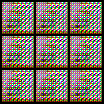
\includegraphics[clip,width=7.0cm]{../../test/images/3100.png}
	    \caption{1epoch 32x32の結果9枚}
	    \label{fig:result}
	  \end{center}
	\end{figure}

	\begin{figure}[htbp]
  	\begin{center}
	    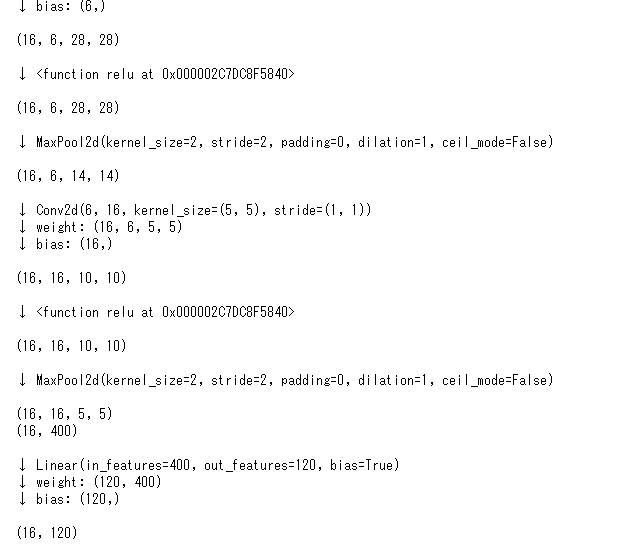
\includegraphics[clip,width=14.0cm]{./ss.png}
	    \caption{モデルのレイヤ情報}
	    \label{fig:helper}
	  \end{center}
	\end{figure}

	% % 参考文献リスト
	% \bibliographystyle{unsrt}
	% \bibliography{2020_04_17}
\end{document}
